


\usetikzlibrary{calc}



\tikzset{
every grid/.style={line cap=rect},
line cap=rect
}



\newcommand{\drawgrid}[2]{%
\draw[line cap=rect] (0,0) grid ++ (#1,#2); 
}

\newcommand{\fillcoord}[2]{%

\fill[black] (#1,#2) rectangle ++ (1,1);

}

\newcommand{\namecoord}[4]{%

\node[label=center:#4] (#3) at ($(#1,#2)+(0.5,0.5)$) {}; 

}


\newcommand{\selectcoord}[2]{%

\draw[color=red, line width=1pt,line cap=rect]  (#1,#2) grid ($(#1,#2)+(1,1)$) {}; 

}




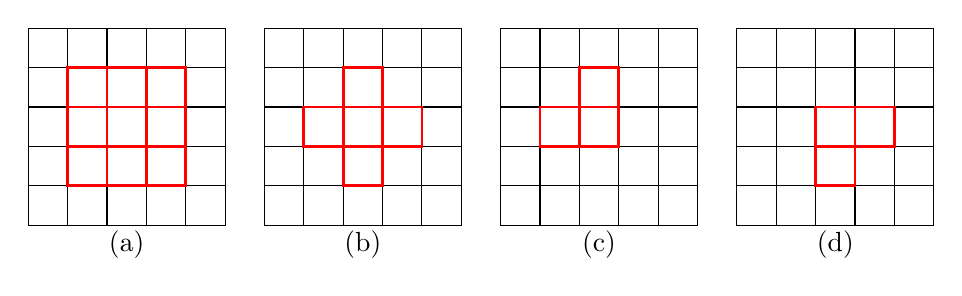
\begin{tikzpicture}[scale=0.5]







\drawgrid{5}{5}



\namecoord{2}{-1}{}{(a)}


\drawgrid{5}{5}

\selectcoord{1}{1}
\selectcoord{2}{1}
\selectcoord{3}{1}

\selectcoord{1}{2}
\selectcoord{2}{2}
\selectcoord{3}{2}

\selectcoord{1}{3}
\selectcoord{2}{3}
\selectcoord{3}{3}





\begin{scope}[shift={(6,0)}]
\namecoord{2}{-1}{}{(b)}



\drawgrid{5}{5}


\selectcoord{2}{1}

\selectcoord{1}{2}
\selectcoord{2}{2}
\selectcoord{3}{2}

\selectcoord{2}{3}


\end{scope}

\begin{scope}[shift={(12,0)}]
\namecoord{2}{-1}{}{(c)}


\drawgrid{5}{5}




\selectcoord{1}{2}
\selectcoord{2}{2}
\selectcoord{2}{3}




\end{scope}

\begin{scope}[shift={(18,0)}]
\namecoord{2}{-1}{}{(d)}




\drawgrid{5}{5}
\selectcoord{3}{2}
\selectcoord{2}{2}
\selectcoord{2}{1}


\end{scope}


\end{tikzpicture}



